\chapter{Metody przetwarzania obrazu i sposoby sterowania w procesie autonomicznego lądowania drona}
%Przegląd systemów wizyjnych wspomagających autonomiczne lądowanie drona
\label{cha:metody}
Wykonywanie różnorodnych scenariuszy misji przez drona wymaga osiągnięcia określonego poziomu autonomii. Bezzałogowy statek powietrzny musi być w~stanie wystartować, nawigować oraz wylądować bez bezpośredniego udziału człowieka. 
Przemieszczanie drona pomiędzy różnymi punktami nawigacyjnymi przebiega bezproblemowo, kiedy dostępny jest sygnał GPS. 
Kłopotu nie~sprawia również start wykonywany bez pomocy operatora (z~ustalonego lądowiska, przy braku przeszkód terenowych). 
Potencjalnie największe wyzwanie stanowi autonomiczne lądowanie drona. 
Platforma obliczeniowa wraz z~zespołem sensorów zainstalowana na~statku powietrznym musi być w~stanie wykryć lądowisko oraz wysłać odpowiednie sygnały sterujące. 
Efektem działania algorytmu sterującego musi być zajęcie dogodnej pozycji do~obniżenia lotu i~ostatecznie przyziemienie w~określonym punkcie. \\
Zadania autonomicznego lądowania drona można podzielić na~dwie kategorie:  
\begin{itemize}
	\item lądowanie na~platformie pozostającej w~bezruchu względem ziemi,
	\item lądowanie na~poruszającej się platformie.
\end{itemize}

W przypadku lądowania na oznaczonym stacjonarnym lądowisku, głównym problemem jest skuteczna detekcja znacznika oraz jego śledzenie. 
Do realizacji tego zadania niezbędne jest wykonanie szeregu kroków.
Przykładowe rozwiązanie z~pracy \cite{Rings} obejmuje:
\begin{itemize}
	\item zamianę obrazu kolorowego na obraz w~skali szarości,
	\item binaryzację ze stałym progiem,
	\item indeksację,
	\item odrzucenie obiektów o~liczbie pikseli mniejszej niż zadany próg,
	\item identyfikację znacznika.
\end{itemize}

Wartości progów binaryzacji oraz odrzucenia małych obiektów zostały dobrane eksperymentalnie. 
Aby dodatkowo wyeliminować biały szum oraz zakłócenia typu ,,sól i~pieprz'' w~pracy \cite{H_median} wprowadzono operację mediany z~oknem 3x3 na obrazie w skali szarości. 
Dodatkowo zastosowano ograniczenie na maksymalny rozmiar obiektu. 
W~algorytmie przedstawionym w pracy \cite{FPGA} binaryzacji dokonano w~przestrzeni barw HSV (ang. \textit{Hue Saturation Value}), na~podstawie składowych S~i~V. 
Pozwoliło to na przeprowadzenie segmentacji niezależnej od koloru (barwy). 
Przed rozpoznawaniem kształtów, na~obrazie binarnym dokonano kolejno erozji oraz dylatacji, co  pozwoliło na eliminację z~obrazu małych grup pikseli. \par 

Istotnym elementem planowania autonomicznego lądowania drona jest wybór znacznika lądowiska. 
W~pracy \cite{Falanga} przedstawiono marker złożony z trzech figur: kwadratu, koła i~krzyża. 
Znacznik pokazano na rys.~\ref{fig:znacznik_falanga}. 
\begin{figure}
	\centering
		
		\begin{subfigure}{0.3\textwidth}
		\centering
		
\includegraphics[width=\textwidth]{znacznik_falanga.jpg}
		\caption{Znacznik użyty w pracy \cite{Falanga}}
		\label{fig:znacznik_falanga}
		\end{subfigure}%
		\begin{subfigure}{0.3\textwidth}
		\centering
		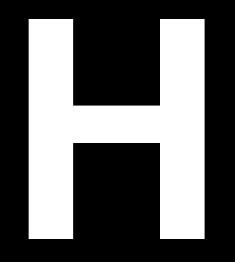
\includegraphics[width=0.9\textwidth]{znacznik_H.jpg}
		\caption{Znacznik użyty w pracy \cite{H}}
		\label{fig:znacznik_H}
		\end{subfigure}
		\begin{subfigure}{0.3\textwidth}
		\centering
		
\includegraphics[width=\textwidth]{znacznik_rings.jpg}
		\caption{Znacznik użyty w pracy \cite{Rings}}
		\label{fig:znacznik_rings}
		\end{subfigure}
	\caption{Porównanie znaczników użytych w pracach \cite{Rings},\cite{Falanga} i \cite{H}}.
	\label{fig:Znaczniki}
\end{figure}

Zaimplementowany został algorytm detekcji lądowiska, który bazował na kolejnym wykrywaniu wymienionych figur, co pozwoliło na coraz lepsze określenie położenia celu.

Prostsze rozwiązanie zostało pokazane w~pracy\cite{H}, gdzie znacznik ma kształt litery \textbf{H} (Rys.~\ref{fig:znacznik_H}) 
Odległość drona od lądowiska obliczana jest na podstawie liczby pikseli dzielących środek ciężkości znacznika od~środka obrazu. 
Opisano tam również metodę wyznaczania orientacji drona względem takiego markera. 
Polega ona na~znalezieniu piksela najbardziej odległego od~środka ciężkości, a~następnie wykreśleniu linii przechodzącej przez te~dwa punkty (punkty F i~G na rys. \ref{fig:pozycja_H_a}).  %TODO2 dopisać, że to punkty F iG ? (wykonane)
Otrzymana linia nie określa jednak pozycji znacznika w~sposób jednoznaczny.
Do~określenia, czy~zachodzi przypadek przedstawiony na~rys. \ref{fig:pozycja_H_a}, czy też \ref{fig:pozycja_H_b}, obliczono kąt $\theta$ pomiędzy dwoma narożnymi punktami (F i~A) markera. %TODO2 Jeśli dobrze to rozumiem tu F i A (wykonane)
Kąt obliczany jest na~podstawie zapisanego obrazu znacznika. 
Następnie wykorzystując znalezioną wcześniej linię, obliczane są współrzędne tych dwóch punktów (punkty A i~B na Rys. \ref{fig:pozycja_H_a}). 
Kolejną czynnością jest sprawdzenie, który z~punktów leży bliżej obszaru markera, czyli litery \textbf{H}. %TODO2 obszar markera, czyli co litera H ? niejasne (wykonane)
Jeśli jest to~punkt~A -- zachodzi przypadek z~Rys.~\ref{fig:pozycja_H_a} i~dron ustawiony jest w~osi znacznika, jeśli B -- Rys.~\ref{fig:pozycja_H_b}.
%TODO2 no a gdzie jest koniec końców ten kąt ?
\begin{figure}
	\centering
	\begin{subfigure}{0.4\textwidth}
		\centering
		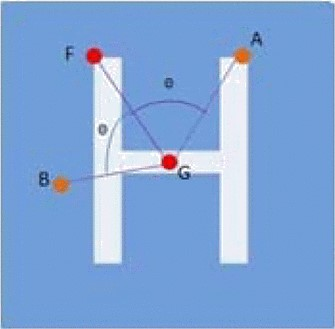
\includegraphics[width=\textwidth]{pozycja_H_a.jpg}
		\caption{}
		\label{fig:pozycja_H_a}
	\end{subfigure}
	\begin{subfigure}{0.4\textwidth}
		\centering
		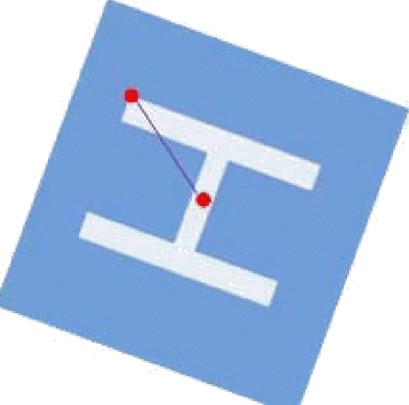
\includegraphics[width=\textwidth]{pozycja_H_b.jpg}
		\caption{}
		\label{fig:pozycja_H_b}
	\end{subfigure}%
	\caption{Ilustracja określania pozycji znacznika w pracy \cite{H} }.
	\label{fig:Znacznik_H_pozycja}
\end{figure}

Inny znacznik został użyty w pracy \cite{Rings}. 
Składa się on z~czterech pierścieni na czarnym tle (Rys.~\ref{fig:znacznik_rings})
Każdy pierścień posiada unikalny stosunek promienia wewnętrznego do zewnętrznego i~stanowi oddzielny obiekt dla systemu wizyjnego. 
Obiekty, które nie mają dokładnie jednej ,,dziury'' wewnątrz, są~pomijane. 
Każdy z~pozostałych jest ostatecznie identyfikowany za pomocą współczynnika kształtu. 
Zaletą takiego znacznika jest możliwość dołożenia kolejnych, większych pierścieni, jeśli lądowisko ma być widoczne z~większej wysokości.


W~procesie autonomicznego lądowania drona, na~podstawie wyznaczonej odległości od celu, do~bezzałogowego statku powietrznego wysyłane są sygnały sterujące. 
W~pracy \cite{Sudevan} wykorzystano trzy regulatory PID, do~kontroli prędkości drona. 
Dzięki nim równocześnie minimalizowana jest każda z~trzech składowych wektora położenia. 
W~pracy \cite{Rings} zwrócono uwagę na błędy spowodowane pochyleniem i~przechyleniem drona. 
Przed wysłaniem sygnału do regulatora wykonywana jest korekta uchybu na~podstawie pomiaru kąta pochylenia i~przechylenia. 
Krok ten był potrzebny z~uwagi na~sztywne umieszczenie kamery na~ramie drona (brak tzw. gimbala). 


W~przypadku wykonywania lądowania na~poruszającej się platformie, do~opisanego wcześniej problemu detekcji znacznika dochodzi również konieczność implementacji bardziej skomplikowanego algorytmu sterowania oraz bardziej niezawodnego śledzenia położenia lądowiska. 
Wysyłane sygnały sterujące muszą uwzględniać ruch lądowiska. 
Przemieszczanie drona powinno nadążać za~zmianą położenia platformy. 
W~takim przypadku układ regulacji jest układem śledzącym.

W~\cite{Falanga} użyto algorytmu pozwalającego na predykcję zachowania celu. 
Wykorzystano dynamiczny model celu oraz rozszerzony filtr Kalmana. 
Na rys.~\ref{fig:trajektorie} przedstawiono schemat wyboru trajektorii. 
System planuje kilka możliwych dróg dotarcia do~lądowiska. 
Każda z~nich ma~początek w~aktualnej pozycji drona, a~kończy się w~przewidzianym położeniu platformy. 
Przyszły stan poruszającego się celu jest określany na~podstawie jego modelu dynamicznego, począwszy od~ostatniej dostępnej estymaty z~filtru Kalmana. 
Trajektorie wymagające sterowania spoza dostępnego zakresu lub kolidujące z~przeszkodami, są odrzucane (trajektoria oznaczona czerwoną przerywaną linią). 
Spośród wszystkich możliwych dróg (niebieskie przerywane linie) wybierana jest ta~wymagająca użycia najmniejszej ilości energii. 
Zadanie optymalizacji jest wykonywane przy wykorzystaniu szybkiej wielomianowej generacji trajektorii minimalizującej trzecią pochodną położenia.
\begin{figure}[h]
	\centering
	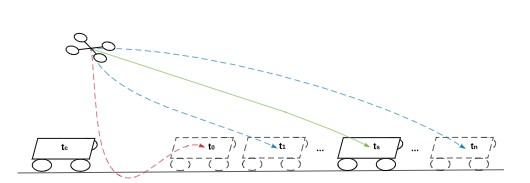
\includegraphics[width=\textwidth]{trajektorie.jpg}
	\caption{Przykład wybierania trajektorii z~pracy \cite{Falanga}.}
	\label{fig:trajektorie}
\end{figure}


Podsumowując, wykonanie lądowania na statycznym lądowisku wymaga skutecznej detekcji znacznika znajdującego się na platformie, który określa jego lokalizację. 
Znalezienie względnej pozycji markera umożliwia przekazanie informacji o~uchybie do~regulatora sterującego dronem. 
Do~urządzenia wykonawczego, czyli silników, dociera ostatecznie informacja o~pożądanej wartości ciągu, która spowoduje zbliżenie do~celu. 
Po~ustabilizowaniu unoszenia drona nad lądowiskiem następuje polecenie stopniowego obniżania lotu, aż~do~zetknięcia z~ziemią.
W~przypadku lądowania na~ruchomym celu nie ma~możliwości doprowadzenia do~zawisu nad platformą. 
Należy zatem przeprowadzić predykcję zachowania lądowiska, wygenerować możliwe trajektorie i~użyć jednej z~metod optymalizacji do~wyboru najlepszej z~nich.

